% A good introduction to latex can be found here:
%    http://www.cse.ohio-state.edu/~hank/latex/lshort141.pdf

\documentclass[9.5pt]{extarticle}

\usepackage{full page}  % make the margins somewhat smaller than the default
\usepackage{graphicx}
\usepackage{amsmath}
\usepackage{indentfirst}
\usepackage{color}
\usepackage{cite}
\usepackage{wasysym}
\usepackage{amssymb}
\usepackage{multirow}
\usepackage{float}
\usepackage{lscape}
\usepackage{alltt} 
\usepackage{listings}
\usepackage{booktabs}
\usepackage{mathtools}
\usepackage{fancyhdr}
\usepackage[table,xcdraw]{xcolor}

\DeclarePairedDelimiter{\ceil}{\lceil}{\rceil}
\DeclarePairedDelimiter{\floor}{\lfloor}{\rfloor}

\definecolor{dkgreen}{rgb}{0,0.6,0}
\definecolor{gray}{rgb}{0.5,0.5,0.5}
\definecolor{mauve}{rgb}{0.58,0,0.82}


\usepackage{listings}  %  needed for source code listings

\lstset{frame=tb,
  language= java,
  aboveskip=1.5mm,
  belowskip=1.5mm,
  showstringspaces=false,
  columns=flexible,
  basicstyle={\small\ttfamily},
  keywordstyle=\color{blue},
  commentstyle=\color{dkgreen},
  stringstyle=\color{mauve},
  breaklines=true,
  tabsize=2,
  numbers=left,
  stepnumber=1,    
  firstnumber=1,
  numberfirstline=true
}
       

% set the document title, author, and date here.
%  once set, the \maketitle command (within the document)
%  will display them nicely
\title{Mazeworld Assignment}
\author{Chua Zheng Fu Edrei}

\begin{document}
\maketitle

\section{Introduction}

In this report, I will implement A* search for robots trying to navigate from a starting location to a goal location in Mazeworld. I will demonstrate the feasibility and optimality of the algorithm by comparing it with breadth-first search (BFS) and depth-first search (DFS) for the problem with one robot. I will also expand the problem to include multiple robots and compare the performance of A* search with other search algorithms. Finally, I will implement a model of a blind robot who doesn't know its original position in the maze and whose goal is to figure out his location in the maze. Additional features will also be discussed.


\section{A-star search}

I implemented A-star search using the algorithm in the textbook (I modified it to discard before the for loop nodes with states that have been visited and have higher priority value than a previous node with the same state). I made use of three data structures: $frontier$ which is Java's implementation of priority queue to keep track of states to visit, $frontierMap$ which is a hash map to store the priority number of the states in frontier, and $reachedFrom$ which is a hash map that maps the current node to the previous node for back chaining. The relevant code is shown in Listing 1.

\begin{lstlisting}[language=java,caption={Java code for A-star search}]
while(!frontier.isEmpty()){
	SearchNode currentNode = frontier.poll();
	if(currentNode.goalTest())
		return backchain(currentNode,reachedFrom);
	else if(frontierMap.containsKey(currentNode) && 		 currentNode.priority()>frontierMap.get(currentNode))
		continue; // discard the node

	for(SearchNode child: currentNode.getSuccessors()){
		if(!frontierMap.containsKey(child) || child.priority() < frontierMap.get(child)){
			reachedFrom.put(child, currentNode);
			frontier.add(child);
			frontierMap.put(child, child.priority());
		}
	}
}
return null;
\end{lstlisting}

I used the suggestion on the canvas assignment instructions of marking items if they have already been visited using a hash map and discarding the node if it has a higher cost than already appears in visited for that state. I also tested the algorithm with 5 different maze layout  - simple.maz (7x7), empty.maz (7x6), rearrange.maz (5x5), tricky.maz (7x5) and large.maz (40x40). The layout for the different type of mazes will be shown in Section 3. As shown in Table 1, A*  is optimal (it produces the shortest path, same as BFS). In terms of run time (measured by the number of nodes explored), A* is superior to both BFS and DFS. In particular, for larger maze (see the last column), A* is a lot more time and space efficient than BFS (A* explored roughly 10 times less nodes and requires half the space of BFS). Note that for large.maz, DFS is not computationally feasible (more on that in Section 3.3).

\begin{table}[H]
\begin{tabular}{@{}cccccccccccccccc@{}}
\toprule
    & \multicolumn{3}{c}{simple.maz}                                                       & \multicolumn{3}{c}{empty.maz} & \multicolumn{3}{c}{rearrange.maz}                                                                                                                         & \multicolumn{3}{c}{tricky.maz} & \multicolumn{3}{c}{large.maz}                                                          \\ \midrule
    & \cellcolor[HTML]{C0C0C0}L  & \cellcolor[HTML]{C0C0C0}T  & \cellcolor[HTML]{C0C0C0}S  & L        & T        & S       & \cellcolor[HTML]{C0C0C0}{\color[HTML]{333333} L}  & \cellcolor[HTML]{C0C0C0}{\color[HTML]{333333} T}  & \cellcolor[HTML]{C0C0C0}{\color[HTML]{333333} S}  & L        & T        & S        & \cellcolor[HTML]{C0C0C0}L  & \cellcolor[HTML]{C0C0C0}T   & \cellcolor[HTML]{C0C0C0}S   \\
BFS & \cellcolor[HTML]{C0C0C0}21 & \cellcolor[HTML]{C0C0C0}24 & \cellcolor[HTML]{C0C0C0}21 & 7        & 27       & 38      & \cellcolor[HTML]{C0C0C0}{\color[HTML]{333333} 11} & \cellcolor[HTML]{C0C0C0}{\color[HTML]{333333} 16} & \cellcolor[HTML]{C0C0C0}{\color[HTML]{333333} 17} & 21       & 24       & 25       & \cellcolor[HTML]{C0C0C0}16 & \cellcolor[HTML]{C0C0C0}136 & \cellcolor[HTML]{C0C0C0}169 \\
DFS & \cellcolor[HTML]{C0C0C0}23 & \cellcolor[HTML]{C0C0C0}23 & \cellcolor[HTML]{C0C0C0}23 & 17       & 17       & 17      & \cellcolor[HTML]{C0C0C0}{\color[HTML]{333333} 13} & \cellcolor[HTML]{C0C0C0}{\color[HTML]{333333} 13} & \cellcolor[HTML]{C0C0C0}{\color[HTML]{333333} 13} & 23       & 23       & 23       & \cellcolor[HTML]{C0C0C0}NA & \cellcolor[HTML]{C0C0C0}NA  & \cellcolor[HTML]{C0C0C0}NA  \\
A*  & \cellcolor[HTML]{C0C0C0}21 & \cellcolor[HTML]{C0C0C0}23 & \cellcolor[HTML]{C0C0C0}46 & 7        & 6        & 27      & \cellcolor[HTML]{C0C0C0}{\color[HTML]{333333} 11} & \cellcolor[HTML]{C0C0C0}{\color[HTML]{333333} 10} & \cellcolor[HTML]{C0C0C0}{\color[HTML]{333333} 35} & 21       & 23       & 46       & \cellcolor[HTML]{C0C0C0}16 & \cellcolor[HTML]{C0C0C0}15  & \cellcolor[HTML]{C0C0C0}72  \\ \bottomrule
\end{tabular}
\centering
\caption{A*, DFS and BFS for simple maze robot problem. L denotes path length (number of turns needed), T denotes run time (number of nodes explored) and S denotes space requirement (maximum space usage). NA denotes that search exceeds the given computational time}
\label{my-label}
\end{table}


\section{Multi-Robot maze}

\subsection{Previous Work (non-graduate student)}

I refer to the work by Standley, T. 2010 (Finding optimal solutions to cooperative pathfinding problems. In The Twenty-Fourth AAAI Conference on Artificial Intelligence (AAAI’10), 173–178). In this paper, Standley presented ``the first practical, admissible, and complete algorithm'' for solving the multi-robot maze. His implementation uses A* search to find an initial path for each agent independently at the beginning by assigning each agent to a group. The basic idea is that sometimes the optimal paths of two agents might conflict and when that happen, an algorithm will perform tie breaking and try to find another optimal path. If alternate optimal paths cannot be found for either agents, the algorithm will collapse both groups into one and will solve for the merged problem. While his algorithm has similar performance to the standard algorithm for small number of agents, the improvement in run time is significant as the number of agents increases and an exponential regression yield $t = 0.465e^{1.14s}$ where $t$ is the run time in $ms$ to solve the problem using his algorithm and $s$ is the number of agents. His approach is interesting because he decomposes the original problem into subproblems (solving for the path of each agent independently), and only merge the subproblems together if there is a conflict, resulting in a more practical algorithm that is at the same time, complete and admissible.

\subsection{Theory and Discussion}

For the multi robot problem, we have $k$ robots in a maze of $n\times n$ located at their respective starting position. The aim is for each robot to move to its goal position. It is possible to represent the state of the system by the location of each robot (its x and y position) and the turn (if we assume that only one robot can move at a time in a given sequence). Therefore, we need $2k + 1$ numbers to represent each state.\\

If we assume no walls inside the maze and ignore collisions, the upperbound for the total number of arrangement of robots can be given as $n^2$ permutates $k$ since we are choosing $k$ locations from $n^2$ possible positions and the ordering matters. In addition, there are $k$ possible turns. Thus, $O(\#state) = \frac{k(n^2)!}{(n^2-k)!}$.\\

To find the number of states that represent collision, we note that if there are $w$ walls, the number of  possible robot location without collision will be $(n^2 - w)$ permutates $k$ instead. Thus $O(\#collide_states) =  \frac{k(n^2)!}{(n^2-k)!} - \frac{k(n^2-w)!}{(n^2-w-k)!}$. Alternatively, if we assume that $k << w$, we can just introduce a scaling factor of $\frac{w}{n^2}$ to find the ratio of state space with collision to the total state space, thus $O(\#collide_states) = \frac{w}{n^2}\frac{k(n^2)!}{(n^2-k)!}$.\\

If there are not many walls and $n$ is large (say $100 \times 100$) and several robots (say 10), I will expect that a straightforward BFS to be computationally infeasible for most start and goal pairs (except for those in which the start and goal pairs are located near each other). This is because if the start and goal pairs are far from each other, BFS will have to go through almost all the states, and we noted previously that the number of states increases with the factorial of $n^2$ (which is even faster than exponential increase!). For $n=100$ and $k=10$, that amounts to $9.96 \times 10^{40}$ number of states!\\

A useful and monotonic heuristic function for this search space will be the summation of the manhattan distance of each robot to its goal state. This heuristic is an underestimate because the shortest distance for each robot to its goal state will be the manhattan distance, and often if there are obstacles along the way, the actual distance will be longer. In addition, due to the triangle inequality, the heuristic will be monotonic too (consider $h(n) \leq c(n,a,n') + h(n')$, note that the manhattan distance will always be less than or equal to the actual distance i.e. $h(n) - h(n') \le c(n,a,n')$).\\

Finally, the 8 puzzle in the book is a special case of the multi robot function because the aim is also for each tile to move from its starting position to the goal position. Our previous heuristic will still be monotonic because if anything, it will be a greater underestimate of the cost. Movement is now restricted to the neighbouring (4,3, or 2 depending on if empty slot is at the center, side or corner) tiles of the empty slot. Each tile needs to move at least its manhattan distance to reach the goal.\\

The state space of the 8-puzzle is made of two disjoint set (one that can be solved to obtain a chronological order of number, and one that could not and each set contains $\frac{9!}{2}$ states) and it is possible to prove using induction. We can also modify our program to prove this by having the start state as the original chronological ordering and by calculating the number of distinct states possible using BFS or DFS until there are no more distinct states left and compare the size of the set with the total number of combination $9!$.

\subsection{Implementation of model}

I implemented the states as a 1D array $int[] state = \{x_1,y_1, ... x_k,y_k,t\}$, where $x_i$ denotes the x-coordinate of the $i^{th}$ robot, $y_i$ denotes the y-coordinate of the $i^{th}$ robot, and $t$ denotes the turn  ($t=i$ denotes that it is the $i^{th}$ robot's turn). Listing 2 shows the implementation of \verb`getSuccessors`. Note that  $2*turnIndex$ in line 6 and $2*turnIndex +1$ in line 7 are used to extract the cooridinate of the robot with the current turn.

\begin{lstlisting}[language=java,caption={Java code for getSuccessors for multi robot maze problem}]
public ArrayList<SearchNode> getSuccessors() {
	ArrayList<SearchNode> successors = new ArrayList<SearchNode>();
	for (int[] action: actions) {
		int[] stateNew  = deepCopy(state);
		int turnIndex = state[state.length-1];
		stateNew[2*turnIndex] = state[2*turnIndex] + action[0];
		stateNew[2*turnIndex+1] = state[2*turnIndex+1] + action[1];
		stateNew[state.length-1] = (turnIndex+1)\%robotNum;
		
		if(maze.isLegal(stateNew[2*turnIndex], stateNew[2*turnIndex+1]) &&
                        !robotCollide(stateNew, stateNew[2*turnIndex], stateNew[2*turnIndex+1])){
			SearchNode succ = new MultiMazeNode(stateNew, getCost() + 1.0);
			successors.add(succ);
		}
	}
	return successors;
}
\end{lstlisting}

The method \verb`deepCopy` creates a deep copy of the original states and the method \verb`robotCollide` checks if the state will result in two robots having the same location. Next, I will present the multi robot A* search for different mazes. Figure 1 shows the movement of 3 robots in simple.maz. This configuration is interesting because we note that the orange piece needs to ensure that it does not stand in the way of the red piece. 

\begin{figure}[H]
\centering
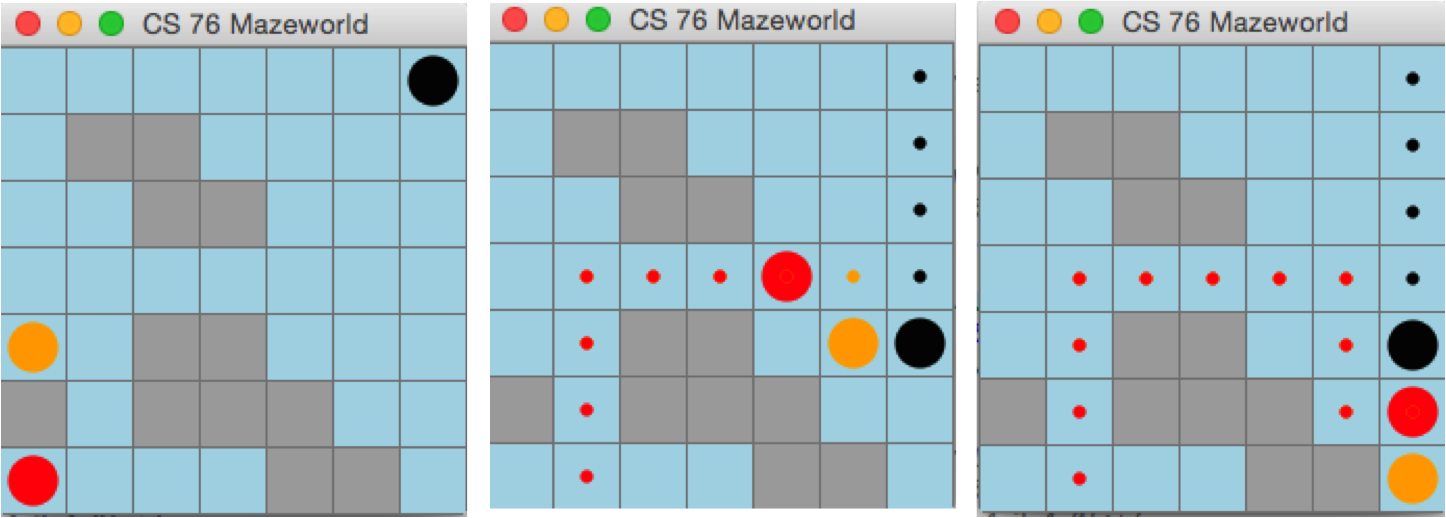
\includegraphics[scale=0.40]{simple_multi.png}
\caption{3 robots in simple.maz. Start state: (0,0), (0,2), (5,5) and goal state is (6,1), (6,0), (6,2) }
\label{Figure 1}
\end{figure}

Figure 2 shows the movement of 3 robots in empty.maz. This configuration is interesting because there is so many degree of freedom, which result in BFS taking a long time  (refer to Table 2 for detailed comparison).

\begin{figure}[H]
\centering
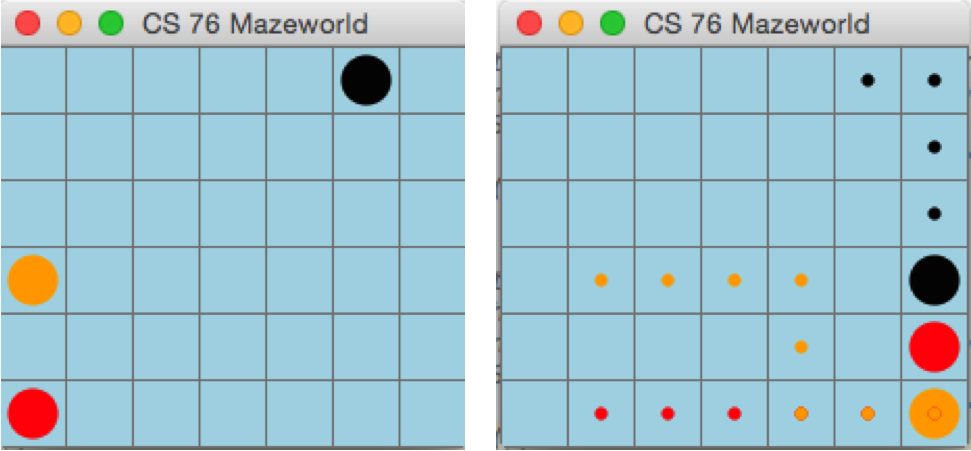
\includegraphics[scale=0.45]{empty_multi.png}
\caption{3 robots in empty.maz. Start state: (0,0), (0,2), (6,6) and goal state is (6,1), (6,0), (6,2) }
\label{Figure 2}
\end{figure}

Figure 3 shows the movement of 3 robots in rearrange.maz. This configuration is interesting because we note that the three pieces need to rearrange among themselves to get to the goal state. This problem cannot be solved by solving for each piece independently since there needs to be some form of coordination.

\begin{figure}[H]
\centering
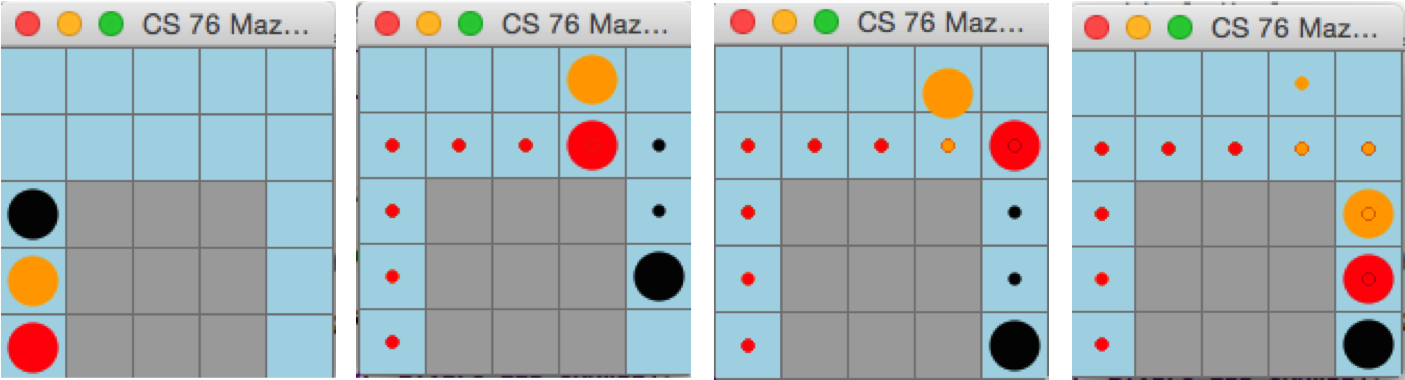
\includegraphics[scale=0.55]{rearrange_multi.png}
\caption{3 robots in rearrange.maz. Start state: (0,0), (0,1), (0,2) and goal state is (4,1), (4,2), (4,0) }
\label{Figure 3}
\end{figure}

Figure 4 shows the movement of 3 robots in tricky.maz. This configuration is the most tricky of all because the narrow alley requires careful coordination between the 3 robots in order to get to the goal state. The figure shows the path of the 3 robots as they try to rearrange themselves with the least number of turns.\\

Figure 5 shows the movement of 2 robots in large.maz. This maze has dimensions $40 \times 40$ (it is being truncated to fit into the page) which means it has a huge state space, making it computationally expensive for BFS to solve (as noted in  section 3.2).


\begin{figure}[H]
\centering
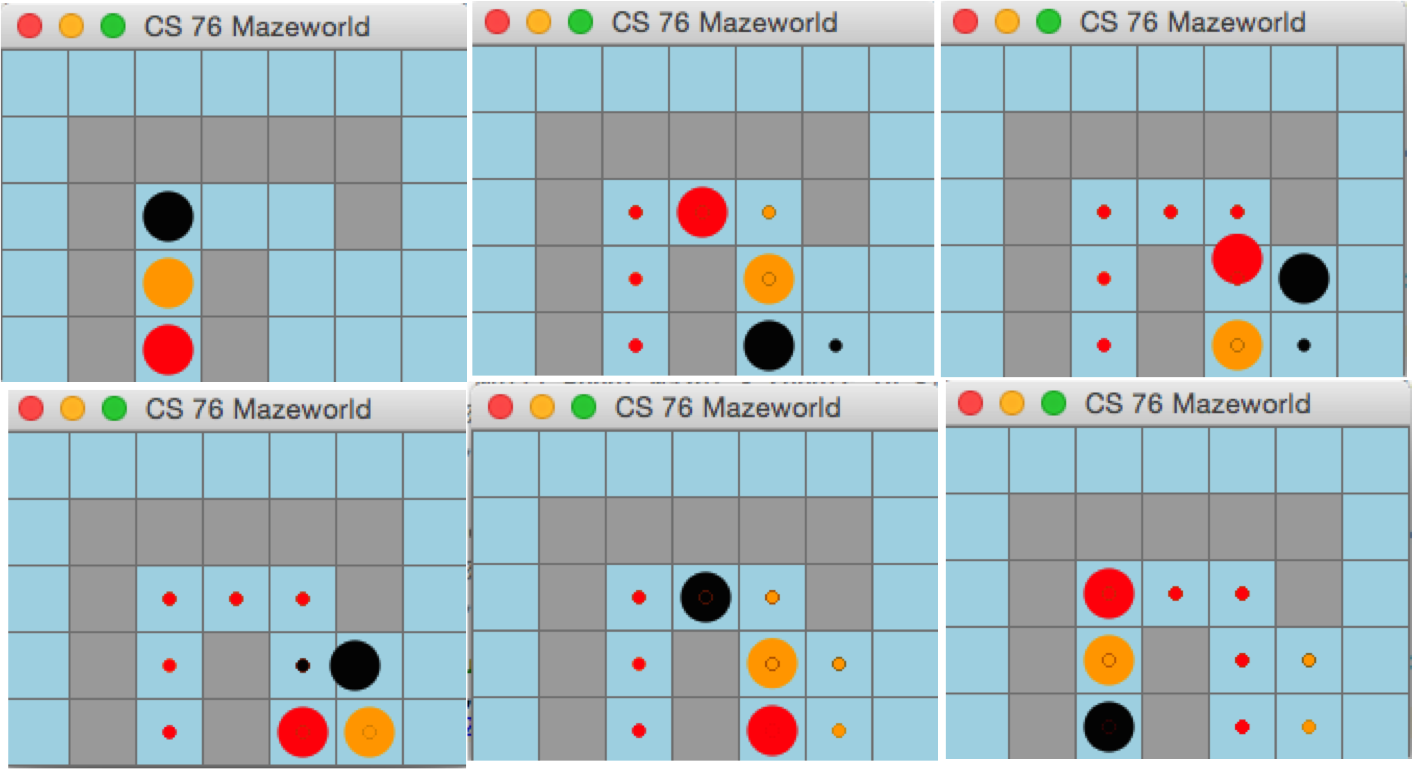
\includegraphics[scale=0.45]{tricky_multi.png}
\caption{3 robots in tricky.maz. Start state: (2,0), (2,1), (2,2) and goal state is (2,2), (2,1), (2,0) }
\label{Figure 4}
\end{figure}

\begin{figure}[H]
\centering
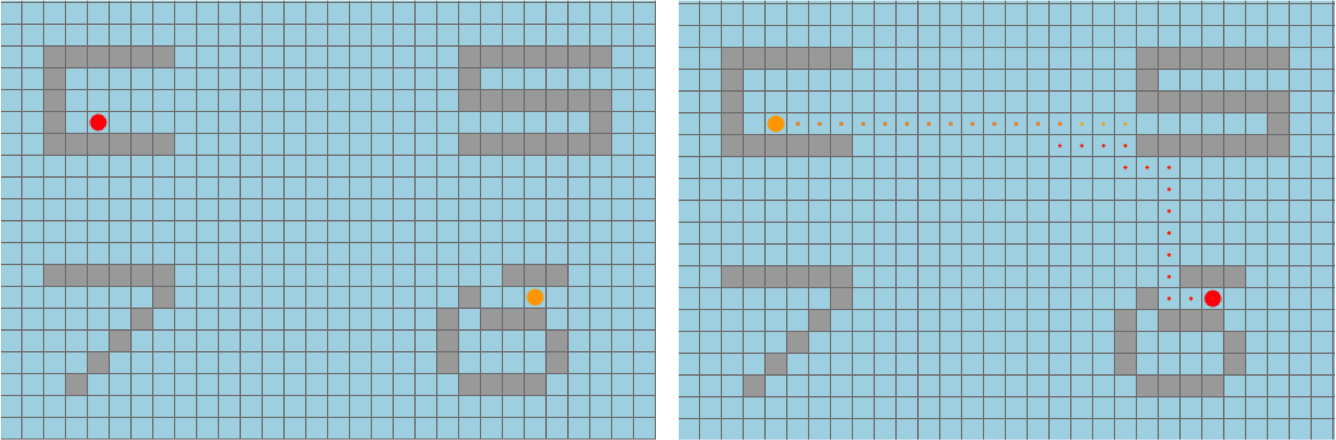
\includegraphics[scale=0.6]{large_multi.png}
\caption{2 robots in large.maz. Start state: (7,32), (27,24) and goal state is (27,24), (7,32) }
\label{Figure 5}
\end{figure}

Table 2 shows the comparison between BFS, DFS and A* for the different mazes. Again, we note that A* is optimal and complete. It is also faster and requires less memory than BFS (the difference gets more significant for larger mazes: more than 1639 times the space requirement and 17755 times the time requirement). Again, DFS is computationally infeasible for tricky and large mazes.

\begin{table}[H]
\resizebox{\textwidth}{!}{%
\begin{tabular}{cccccccccccccccc}

\hline
    & \multicolumn{3}{c}{simple.maz}                                                                   & \multicolumn{3}{c}{empty.maz} & \multicolumn{3}{c}{rearrange.maz}                                                                                                                             & \multicolumn{3}{c}{tricky.maz} & \multicolumn{3}{c}{large.maz}                                                                  \\ \hline
    & \cellcolor[HTML]{C0C0C0}L    & \cellcolor[HTML]{C0C0C0}T        & \cellcolor[HTML]{C0C0C0}S      & L      & T         & S        & \cellcolor[HTML]{C0C0C0}{\color[HTML]{333333} L}  & \cellcolor[HTML]{C0C0C0}{\color[HTML]{333333} T}    & \cellcolor[HTML]{C0C0C0}{\color[HTML]{333333} S}    & L      & T         & S         & \cellcolor[HTML]{C0C0C0}L  & \cellcolor[HTML]{C0C0C0}T       & \cellcolor[HTML]{C0C0C0}S       \\
BFS & \cellcolor[HTML]{C0C0C0}32   & \cellcolor[HTML]{C0C0C0}97164    & \cellcolor[HTML]{C0C0C0}113810 & 24     & 135819    & 161459   & \cellcolor[HTML]{C0C0C0}{\color[HTML]{333333} 33} & \cellcolor[HTML]{C0C0C0}{\color[HTML]{333333} 8978} & \cellcolor[HTML]{C0C0C0}{\color[HTML]{333333} 9599} & 44     & 14644     & 16430     & \cellcolor[HTML]{C0C0C0}57 & \cellcolor[HTML]{C0C0C0}1367188 & \cellcolor[HTML]{C0C0C0}1511281 \\
DFS & \cellcolor[HTML]{C0C0C0}5000 & \cellcolor[HTML]{C0C0C0}76583522 & \cellcolor[HTML]{C0C0C0}5001   & 5001   & 4737183   & 5001     & \cellcolor[HTML]{C0C0C0}{\color[HTML]{333333} NA} & \cellcolor[HTML]{C0C0C0}{\color[HTML]{333333} NA}   & \cellcolor[HTML]{C0C0C0}{\color[HTML]{333333} NA}   & NA     & NA        & NA        & \cellcolor[HTML]{C0C0C0}NA & \cellcolor[HTML]{C0C0C0}NA      & \cellcolor[HTML]{C0C0C0}NA      \\
A*  & \cellcolor[HTML]{C0C0C0}32   & \cellcolor[HTML]{C0C0C0}4960     & \cellcolor[HTML]{C0C0C0}18224  & 24     & 2517      & 13661    & \cellcolor[HTML]{C0C0C0}{\color[HTML]{333333} 33} & \cellcolor[HTML]{C0C0C0}{\color[HTML]{333333} 1205} & \cellcolor[HTML]{C0C0C0}{\color[HTML]{333333} 4468} & 44     & 3698      & 10155     & \cellcolor[HTML]{C0C0C0}57 & \cellcolor[HTML]{C0C0C0}77      & \cellcolor[HTML]{C0C0C0}922     \\ \hline
\end{tabular}
}
\centering
\caption{A*, DFS and BFS for multi maze robot problem. Description of parameters similar to Table 1.}
\label{my-label}
\end{table}

\section{Blind Robot with Pacman physics}
\subsection{Model and Implementation}

The next implementation considers a blind robot in a maze trying to figure out its original position. Note that this problem is very similar to vacuum world described in the book, except that it is deterministic. The basic idea is as follows: if the robot moves North from its orginal position, it knows that its start state cannot possibly be the northern most row. By carefully planning the transition, the number of possible locations will decrease since some locations collapse into each other. The goal of A* is to discover the path that makes all the possible locations collapse.\\

I represent the states in a two dimensional boolean array that is the same dimension as the maze (it is memory expensive but the code looks a lot cleaner and I think the tradeoff is worth it. A more memory efficient data structure will be a bitset). The implementation for \verb`getSuccessors` for the blind robot maze problem is given in Listing 3.

\begin{lstlisting}[language=java,caption={Java code for getSuccessors blind robot maze problem}]
public ArrayList<SearchNode> getSuccessors() {
	ArrayList<SearchNode> successors = new ArrayList<SearchNode>();
	for (int[] action: actions) {
		int xNew = x + action[0];
		int yNew = y + action[1];

		if(maze.isLegal(xNew, yNew)) {
			boolean[][] prevstate = deepCopy(state);
			int xdiff = Math.abs(xNew - xoriginal);
			int ydiff = Math.abs(yNew - yoriginal);
			int decrement = 0;
			SearchNode succ;

			if(Arrays.equals(action,Maze.EAST)){
				 // previous location can't be at the eastern most state
				if(xNew - xoriginal > 0 ) // only make changes if we are not backtracking
						decrement = nullifyCol(mostEast - xdiff + 1, prevstate);
				 succ = new BlindMazeNode(prevstate,xNew, yNew, getCost() + 1.0,numPossible-decrement, "E");
			}else if(Arrays.equals(action,Maze.WEST)){
				//...previous location can't be at the western most state (refer to BlindMazeProblem.java)
			}else if(Arrays.equals(action,Maze.NORTH)){
				 //...previous location can't be at the northern most state (refer to BlindMazeProblem.java)
			}else{
				//...previous location can't be at the southern most state (refer to BlindMazeProblem.java)
			}
			successors.add(succ);
		}
	}
	 return successors;
}
\end{lstlisting}

I then performed A* search for the blind robot model on 5 different mazes. The output is given in Listing 4 with the directions taken. Note that the output for large.maz is not included because the maze is too large and it ran out of memory (due to data structure used).\\

The heuristic used for A* search is the number of possible locations divided by $n$ i.e. $h = numPossible / n$. This heuristic will certainly be an underestimate of the number of moves required to achieve the goal state. Note that in an empty maze of $n \times n$ starting at (0,0), the total number of moves required to collapse all the possible locations to just one location is $2n$. Each time we arrive at a x-coordinate or y-coordinate for the first time, we eliminate a column or row from the possible locations. Therefore, the maximum number of states that can be reduced at each move is $n$. \\

Another possible heuristic that can be used is the total number of unique x-coordinate and y-coordinate left in the set of possible locations (so that at the beginning, the heuristic will yield $2n$). We can keep track of the number of unique x and y values using a hashset. This heuristic will be a better estimate of the number of moves required and thus, will result in a more optimal A*-search. However, the tradeoff is that we have to keep another data structure and this might result in more memory required.

\begin{lstlisting}[language=java,caption={Output for A* search of blind robot model for tricky.maz}]
Blind Robot Maze: Empty Maze
    Start -> W -> W -> E -> E -> N -> N -> E -> E -> E -> N -> E -> N -> N ->  End
    Number of turns: 14; Nodes explored during search:  1210508; Maximum space usage: 11654236
Blind Robot Maze: Simple Maze
    Start -> W -> N -> N -> N -> W -> E -> E -> E -> E -> E -> N -> E -> N -> N ->  End
    Number of turns: 15; Nodes explored during search:  15927; Maximum space usage: 113868	
Blind Robot Maze: Tricky Maze
    Start -> N -> N -> E -> E -> S -> E -> E -> N -> N -> N -> W -> W -> W -> W -> W -> W ->  End
    Number of turns: 17; Nodes explored during search:  21155; Maximum space usage: 130927
Blind Robot Maze: Rearrange Maze
    Start -> N -> N -> N -> N -> E -> E -> E -> E ->  End
    Number of turns: 9; Nodes explored during search:  94; Maximum space usage: 644
\end{lstlisting}

Figure 6 shows the animation for A* search for the blind robot in tricky.maz and the direction plan is included in Listing 4. Note that whenever the robot encounters a new y-coordinate, a row is eliminated and whenever it encounters a new x-coordinate, a column is eliminated. The possible locations at each stage is denoted by the opaque tiles, which becomes translucent when it is removed from the set of possible locations. Also note that the number of possible locations never increases at each stage (it can remain the same, and this happen when it explore a x-coordinate or a y-coordinate that has already been explored).\\

\begin{figure}[H]
\centering
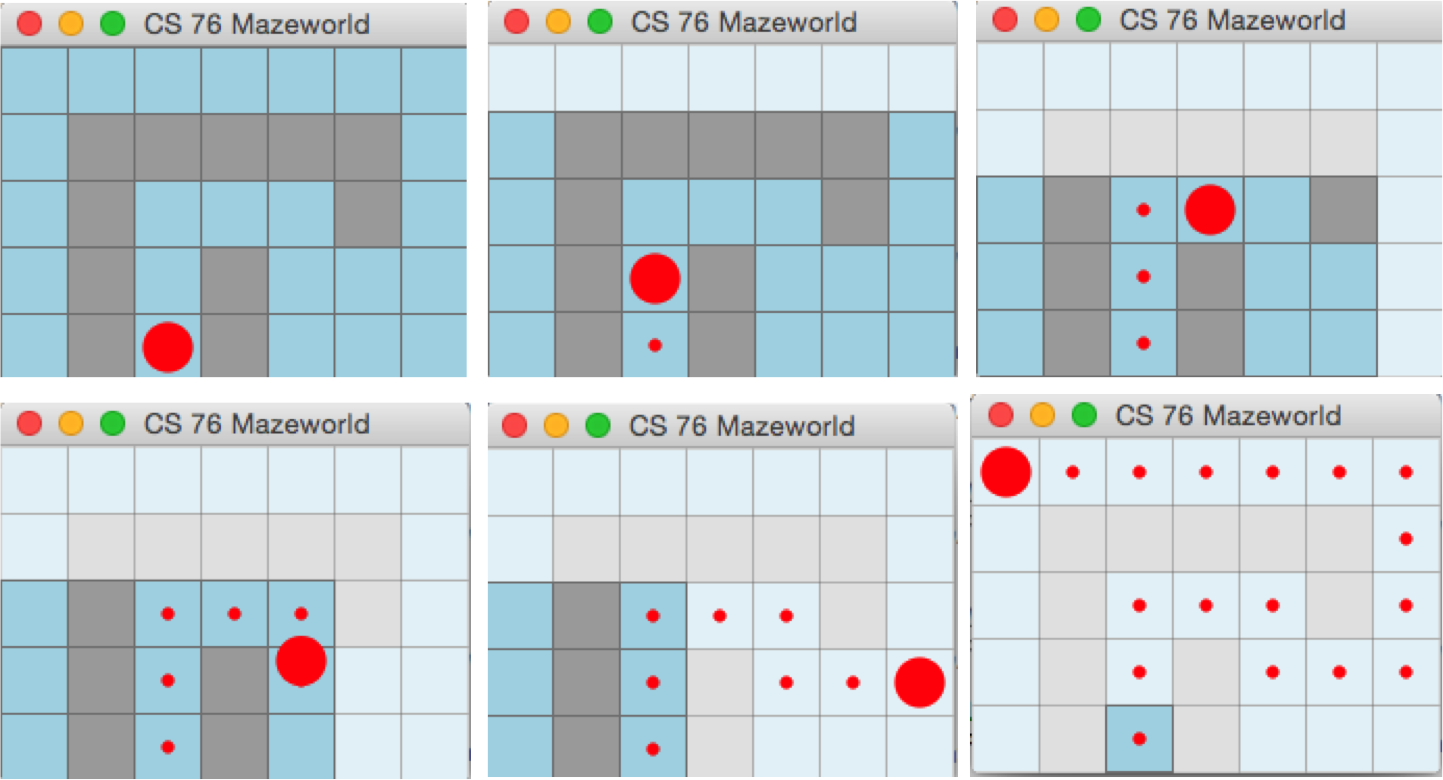
\includegraphics[scale=0.5]{tricky_blind.png}
\caption{Blind robot in tricky.maz }
\label{Figure 5}
\end{figure}

\section{Extra credit}

\subsection{Polynomial-time blind robot planning}

Figure 7 shows the optimal strategy for various mazes. Note that as long as the robot is able to access the set of all unique x-values and y-values (there are $2n-2$ of those for a $n\times n$ maze since we exclude the starting position) i.e. the maze is finite and the goal is in the same connected component of the maze as the start, a solution exists. The proof is as such: whenever the robot encounters a new x-value, it eliminates a new column and whenever it encounters a new y-value, it eliminates a new row. Since we have to exclude the starting position of the robot as the robot can only sense difference in x and y coordinate from it starting position and not absolute coordinates (its starting position is set as potential zero for all other relative measurement), if the robot has access to $n-1$ possible x-values and $n-1$ possible y-values, it will necessarily eliminate $2n- 2$ rows and columns, leaving only one possible location.

\begin{figure}[H]
\centering
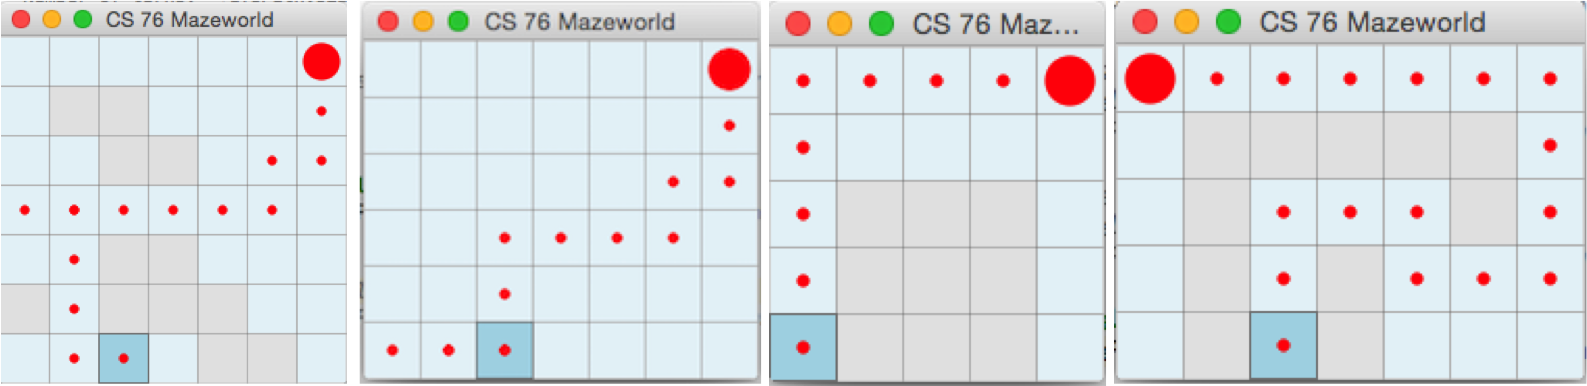
\includegraphics[scale=0.5]{together_blind.png}
\caption{Blind robot in simple.maz, empty.maz, rearrange.maz and tricky.maz (left to right) }
\label{Figure 5}
\end{figure}

A polynomial algorithm is possible: the robot should follow the wall or the outer boundary of the maze on the right side (if the robot has not encounter a wall or the boundary, it will just keep moving straight). This is similar to the right-hand rule for maze search. By doing this, the robot must be able to access all $2n-2$ x-values and y-values if the goal is in the same connected component of the maze as the start. This has quadratic run time since in the worse case, the robot will visit all $n^2$ tiles.

\subsection{Optimizing A* search by tie breaker}

I attempted to optimize A* search by following the suggestion of the TA on piazza to implement a tie-breaking rule: when there are two search nodes with the same priority, A* search would choose the node with the higher heuristic, since that state is closer to the goal. The code is given in Listing 5. I tested the tie-breaking rule with tricky.maz for the multi robot and blind robot problem. Without tie breaking, the multi robot explored 4392 nodes and requires 11886 memory usage; with tie-breaking, the values are 3698 and 10155 respectively. Similarly for the blind robot, the results are 21164 vs 21155 nodes explored and 130963 vs 13097 memory usage, showing that the tie breaking rule is more optimal.

\begin{lstlisting}[language=java,caption={Output for A* search of blind robot model for tricky.maz}]
public int compareTo(SearchNode o) {
	if(priority() > o.priority()){ 
		return 1;
	}else if (priority() < o.priority()){
		return -1;
	}else{ // tie breaker
		if(heuristic() > o.heuristic())	return 1;
		else if(heuristic() < o.heuristic())	return -1;
		else	return 0;
	}
}
\end{lstlisting}

\subsection{Additional graphics}

I implemented the method \verb`addFootPrint` in MazeView.java to show the movement of the robot and the method \verb`updateColor` to make the eliminated location tiles for the blind robot translucent.

\subsection{Literature review}

I did the optional literature review on work by Standley, T. 2010 (refer to section 3.1).





\end{document}